
\documentclass[11pt]{article}

\usepackage{common}
\usepackage{url}
\usepackage{graphicx}
\graphicspath{ {images/} }

\title{HW1: Text Classification}
\author{Alex Saich \\ asaich@college.harvard.edu \and Colton Gyulay \\ cgyulay@college.harvard.edu }
\begin{document}

\maketitle{}
\section{Introduction}

For the first assignment of CS287 we are tasked with text classification, specifically within the realm of movie reviews. Our primary dataset consisted of short strings of words each labeled with a rating in the range $1- 5$. These ratings correspond to each reviewers' sentiment in regard to the film, where lower ratings correspond generally to negative language.

We utilized three different models to learn the statistical associations between specific vocabulary and sentiment. These include a naive Bayes model \citep{murphy2012machine}, a logistic regression model, and a linear support vector machine \citep{wang2012baselines}. The naive Bayes model learned the underlying class distribution and token distribution within these classes, which was then used to predict ratings on examples. The logistic regression and linear SVM models were trained using mini-batch stochastic gradient descent. We experimented with k-fold cross-validation as an improvement over standard methods.

\section{Problem Description and Model}

\subsection{Dataset}

Our data initially came in the format of a string of words (for example, "undeniably fascinating and playful fellow") associated with a class \textit{y} in the range $1- 5$. The total set of vocabulary $\mcV$ seen across training examples included around $17000$ words. We converted each example to a vector $\boldx_{\scriptscriptstyle 1\times \mcV}$ where each index represented the number of occurrences of a specific token within that example.

\subsection{Naive Bayes}

For the naive Bayes model, we first compiled a prior probability vector $\boldy_{\scriptscriptstyle 1\times y}$ to model $P(y)$. We then built a class-word probability matrix $\boldM_{\scriptscriptstyle y\times \mcV}$ that indicates the probability that a word is associated with a given class; $\boldM$ models $P(x|y)$. To avoid zeroing out probabilities of examples with words not seen in a specific class, we add a smoothing constant $\alpha$ to each occurrence count. By an assumption of independence among words in an individual example and by Bayes' theorem, we can treat the probability that an example belongs to a class as proportional to the product of the individual word probabilities and the prior probability of that class. More formally, $p(y_{\scriptscriptstyle i}|x) \propto  p(y_{\scriptscriptstyle i}) \times p(x|y_{\scriptscriptstyle i})$, where $p(x|y_{\scriptscriptstyle i}) = \prod_{j=1}^{\mcV} p(x_{j}|y_{\scriptscriptstyle j})$ from $\boldM$.

\subsection{Logistic Regression and Linear SVM}

Our logistic regression and Linear SVM models use similar topologies and training methods, though differ in cost and gradient calculation. Both models were trained using mini-batch stochastic gradient descent with mini-batch size \textit{m}. A weight matrix $\boldW_{\scriptscriptstyle \mcV\times y}$ and bias vector $\boldb_{\scriptscriptstyle 1\times y}$ were combined in the form $\boldx\boldW + \boldb = \boldz$ and then passed to a Softmax function to convert scores to a normalized probability distribution $\hat{y}_i$ for each class $y_i$. A model's prediction for any example is given by $argmax_i(p(y_i|x))$.

The logistic regression model sought to minimize a cross-entropy loss objective for clarity in this formulation, $c$ represents the correct class: $L_{cross-entropy}(\boldy, \hat{\boldy}) = -\sum_{c} \hat{\boldy_c} log(\hat{\boldy_c})$. Gradients for computing $\frac{\partial L(\boldy, \hat{\boldy_i})}{\partial \boldz_i}$ took the following form, which calculates how the loss varies in regard to the Softmax output $\boldz$:

\[\hat{\boldg} = \left\{
\begin{array}{ll}
      -(1 - \hat{\boldy_i}) & i = y \\
      \hat{\boldy_i} & ow. \\
\end{array}
\right. \]

The gradient for $\boldb$ is simply $\hat{\boldg}$, while the gradient for $\boldW$ is given by $\boldx\hat{\boldg}$. The linear SVM model sought to minimize a hinge loss objective (for clarity in this formulation, $c$ represents the correct class and $c^\prime$ the highest scoring \textit{incorrect} class): $L_{hinge}(\boldy, \hat{\boldy}) = max\{0, 1 - (\hat{\boldy_c} - \hat{\boldy_{c^\prime}})\}$ Gradients for computing  $\frac{\partial L(\boldy, \hat{\boldy})}{\partial \hat{\boldy_j}}$ took the following form:

\[\hat{\boldg} = \left\{
\begin{array}{ll}
      0 & \hat{\boldy_c} - \hat{\boldy_{c^\prime}} > 1 \\
      1 & j = c^\prime \\
      -1 & j = c \\
      0 & ow. \\
\end{array}
\right. \]

The gradients for $\boldb$ and $\boldW$ follow the same pattern as described above. For both regressions, we used $L2$ regularization to prevent overfitting with a regularization coefficient represented by $\lambda$. In our gradient descent, we use a learning rate of $\alpha$ that determines how descent step size. The propagation of these gradients is explained further through pseudo-code in the following \textbf{Algorithms} section.

\section{Algorithms}

The learning using the naive Bayes classifier and the two regressions was done slightly differently. In the case of the naive Bayes, a prior probability of each class' totals was created out of the training data, and then a count matrix for words present in each class. $\boldb$ and $\boldW$ were then normalized to represent probabilities, and new $x$ vectors would be transformed by the weights to find a class distribution. A more in-depth explanation is outlined in pseudo-code below.

The regressions were used mini-batch gradient descent. Because our training set was so large, and because regression inherently takes much longer to train than naive Bayes (gradient weights must be calculated at each step rather than just calculating occurrence sums), we would take randomized batches of the training data for learning. While this meant that the chances of training again on the same datapoint were not 0, we found it was the most efficient way of sampling a subset of the dataset that did not sacrifice our performance. For each mini-batch, an aggregated weight gradient matrix and bias gradient term were created and then applied to our $\boldW$ and $\boldb$. Performing descent in batches rather than stochastically was more efficient because it meant that derivatives only needed to be found every $n$ inputs rather than every time.

We also tried running the regression using k-fold cross-validation (not mentioned in pseudo-code below) in order to see if this would yield a more accurate result. We split the group into $k$ groups, iterating through the groups and holding each of them apart as a validation set while the algorithm trained on the other $k-1$ sets. The weights were then averaged across the $k$ iterations to give a model that better represents all the data. Listed below is pseudo-code for our the algorithms that did the heavy lifting: naive Bayes and SGD. We also include code for the cross-entropy and hinge loss objectives.

\begin{algorithmic}[1]
  \Procedure{Naive Bayes}{$x_1\ldots x_N$, $y_1\ldots y_N$}
  \State{$W \gets 0$}
  \State{$b \gets 0$}
  \For{$i = 0, \ldots, C$}
    \State{$b_c \gets \sum_{i=1}^{n}{\frac{\mathbf{1}(\mathbf{y_i} = c)}{n}}$}
    \State{$F_f \gets \sum_{i=1}^{n}\mathbf{1}(\mathbf{y_i} = c)\mathbf{1}(x_{i,f} = 1)$ for all $f \in F$}
    \State{$W_c \gets \frac{F_f}{\sum_{f' \in F}{F_{f',c}}} $ for all $f \in F$}
  \EndFor{}

  \State{\Return{$W$, $b$}}
  \EndProcedure{}
\end{algorithmic}

  \begin{algorithmic}[1]
    \Procedure{Mini-batch Gradient Descent}{$x_1\ldots x_N$, $y_1\ldots y_N$, $S$, $\alpha$, $\lambda$, $f$}
    \State{$W \gets 0$}
    \State{$b \gets 0$}
    \For{$s = 0, \ldots, S$}
    
    \State{$\vec{X}^{\,} = x_s,\ldots,x_{s+\frac{N}{S}}$}
    \State{$\vec{Y}^{\,} = y_s,\ldots,y_{s+\frac{N}{S}}$}
    \State{$L_2 = \frac{\lambda}{2} \|W\|^2_2$}
    \State{$\hat{y} = WX + b$}
    \If{$f = $ cross entropy}
    \State{$z = $ $\frac{exp(\hat{y})}{\sum_{c}exp(\hat{y_c})}$}
    \State{$\frac{\partial L}{\partial z}$ = crossentropy($z$)}
    \ElsIf{$f$ = hinge}
    \State{$\frac{\partial L}{\partial y}$ = hinge($\hat{y}$)}
    \EndIf{}
    \State{$\frac{\partial L}{\partial b}$ = $\frac{\partial L}{\partial y}$}
    \State{$\frac{\partial L}{\partial W}$ = $x\frac{\partial L}{\partial y}$}
    \State{$b \gets b - \alpha(\frac{\partial L}{\partial b} + \lambda b) $ }
    \State{$W \gets W - \alpha(\frac{\partial L}{\partial W} + \lambda W) $ }
    \EndFor{}
    \State{\Return{$W$, $b$}}
    \EndProcedure{}
  \end{algorithmic}
  
  \begin{algorithmic}[1]
    \Procedure{Cross Entropy}{$\hat{Y}_{1,\ldots,N}$,
    $Y_{1,\ldots,N}$}
    \State{$\frac{\partial L}{\partial y} \gets 0$}
    \For{$i=0, \ldots, N$}
    \State{$\frac{\partial L}{\partial z}_{i,c} \gets -(1 - \hat{y}_i)$}
    \State{$\frac{\partial L}{\partial z}_{i,c'} \gets \hat{y}_i$}
    \EndFor{}
    \State{\Return{$\frac{\partial L}{\partial y}$}}
    \EndProcedure{}
  \end{algorithmic}
    
  \begin{algorithmic}[1]
    \Procedure{Hinge Loss}{$\hat{Y}_{1,\ldots,N}$,
    $Y_{1,\ldots,N}$}
    \State{$\frac{\partial L}{\partial y} \gets 0$}
    \For{$i=0, \ldots, N$}
    \If{$\hat{Y}_{i,c} - \hat{Y}_{i,c'} > 1$}
    \State{$\frac{\partial L}{\partial y}_i \gets 0$}
    \Else{}
    \State{$\frac{\partial L}{\partial y}_{i,c} \gets -1$}
    \State{$\frac{\partial L}{\partial y}_{i,c'} \gets 1$}
    \EndIf{}
    \EndFor{}
    \State{\Return{$\frac{\partial L}{\partial y}$}}
    \EndProcedure{}
  \end{algorithmic}

\section{Experiments}

We found that our results performed considerably better than a baseline model with no learned weights, confirming that our model was in fact learning on the dataset. Between the three distinct models we did not find a wild divergence, as all three performed reasonably well, though the vanilla logistic regression model might have performed better with further hyperparameter tuning. For its simplicity, the naive Bayes model performed impressively. Regression with at least a few passes over the entire dataset performed comparably. All scores reported in Table 1 are based on validation accuracy.

\begin{table}[h]
\centering
\begin{tabular}{llr}
 \toprule
 Model & SST1 & SST2 \\
 \midrule
 \textsc{Naive Bayes} & 39.9 & 80.1  \\
 \textsc{Logistic Regression} & 38.44 & 81.2 \\
 \textsc{Linear SVM} & 40.9 & 77.4 \\
 \textsc{Logistic with 10-fold CV} & 35.8 & 78.8 \\
 \bottomrule
\end{tabular}
\caption{\label{tab:results} Results on datasets SST1 \& SST2}
\end{table}

We've also included plots showing training and validation accuracy over epochs for the logistic regression and linear SVM models. These scores are recorded on the SST1 dataset. Epoch 0 represents prediction accuracy prior to any training.

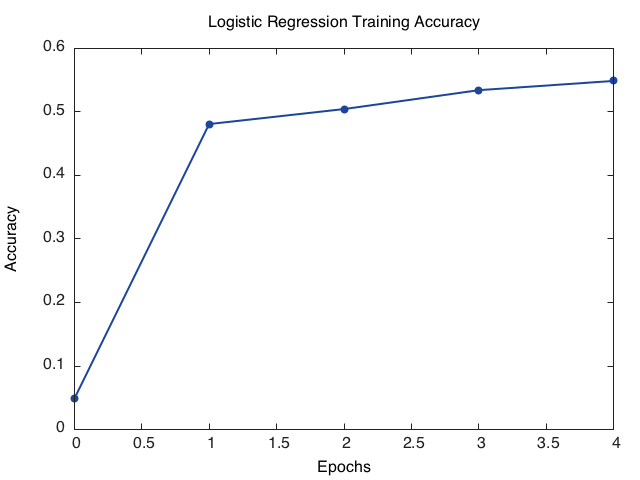
\includegraphics[scale=0.33]{lr_train_sst1}
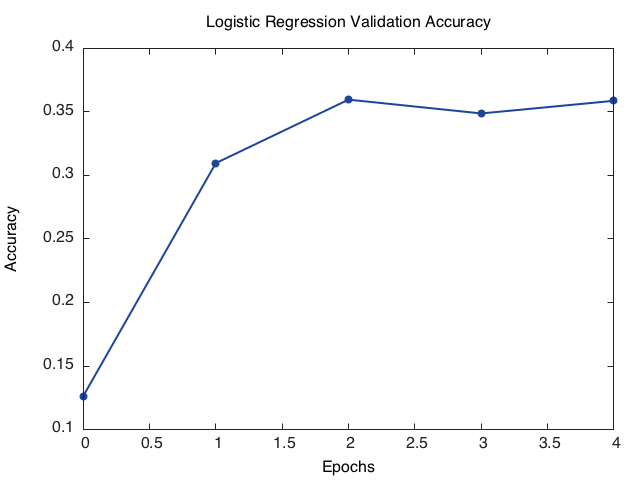
\includegraphics[scale=0.33]{lr_valid_sst1} \\

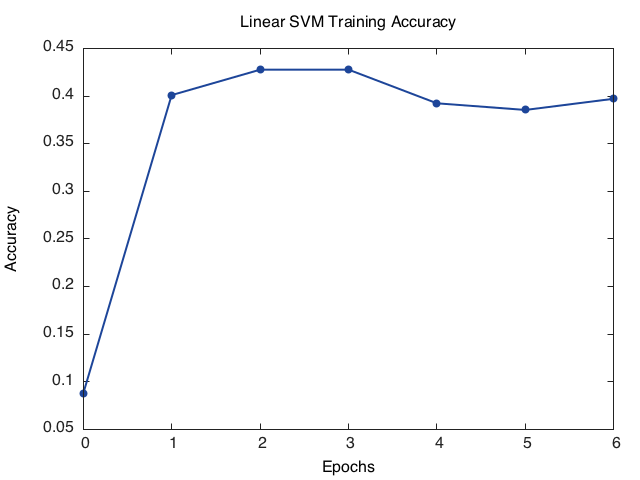
\includegraphics[scale=0.33]{svm_train_sst1}
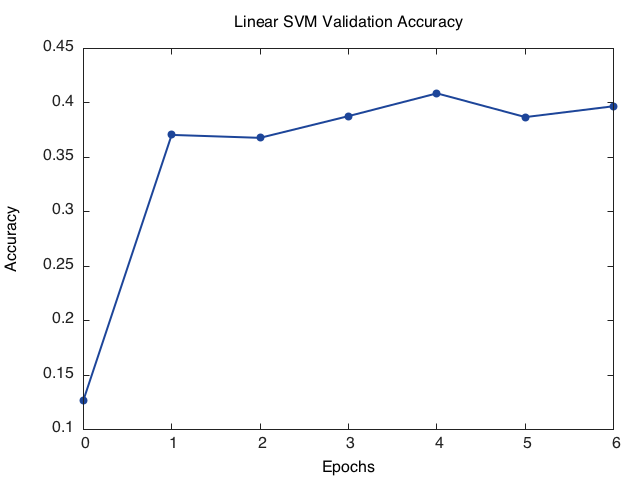
\includegraphics[scale=0.33]{svm_valid_sst1}

\section{Conclusion}

Our final resulting accuracy was on par with others in the class in regard to Kaggle submission. Our models vastly outperformed our baseline performance, and we found that we had the most success with cross-entropy logistic regression (although naive Bayes was the fastest). Furthermore, we found pronounced success using k-fold cross-validation to complement the learning in our mini-batch gradient descent.

We encountered problems with our loss functions as well as trying to get our weights to converge. Our SVM loss at times diverged into the hundreds unless a large $L2$ value was set, despite the fact that our accuracy was continually improving. This could point towards overfitting on our training model given how weight accumulation. Given more time we would have liked to resolve this issue in order to keep the weights and loss lower.

Some additional steps that could have been taken include the implementation of bigrams for inputs, which has been shown to produce better performance and more accurate results. The downside of this, however, would have been the drastic increase in vocabulary size ($\|V\|^2$, all possible combinations of words present). Our limited processing power was already struggling with the size of the massive sparse matrices. We would have also liked to have optimized our sparsify function to run without for-loops, as we found that the run-time of the function was limiting the scope of the dataset that could be used at one time. Since we were using mini-batch SGD, however, this problem was actually not too pronounced. In total, we were able to produce fairly effective models without extensive manual feature engineering. The full source code can be found on GitHub: \url{https://github.com/cgyulay/cs287}.

\bibliographystyle{apalike}
\bibliography{writeup}

\end{document}
